% \documentclass[11pt]{article}
% \usepackage[utf8]{inputenc}	% Para caracteres en español
% \usepackage{amsmath,amsthm,amsfonts,amssymb,amscd}
% \usepackage{multirow,booktabs}
% \usepackage[table]{xcolor}
% \usepackage{fullpage}
% \usepackage{lastpage}
% \usepackage{enumitem}
% \usepackage{fancyhdr}
% \usepackage{mathrsfs}
% \usepackage{wrapfig}
% \usepackage{setspace}
% \usepackage{calc}
% \usepackage{multicol}
% \usepackage{cancel}
% \usepackage[retainorgcmds]{IEEEtrantools}
% \usepackage[margin=3cm]{geometry}
% \usepackage{amsmath}
% \newlength{\tabcont}
% \setlength{\parindent}{0.0in}
% \setlength{\parskip}{0.05in}
% \usepackage{empheq}
% \usepackage{framed}
% \usepackage[most]{tcolorbox}
% \usepackage{xcolor}
% \colorlet{shadecolor}{orange!15}
% \geometry{margin=1in, headsep=0.25in}

\documentclass[11pt]{article}
 
\usepackage[margin=1in]{geometry} 
\usepackage{amsmath,amsthm,amssymb,scrextend}
\usepackage{fancyhdr}
\usepackage{graphicx}
\setlength{\headheight}{14pt}
\usepackage{xcolor}
\usepackage{color,soul}
\usepackage{gensymb}
\pagestyle{fancy}


\begin{document}
 
% --------------------------------------------------------------
%                         Start here
% --------------------------------------------------------------

\lhead{EE267 Virtual Reality}
\chead{Homework 4 Answers}
\rhead{Bohan Li}

\section{Theoretical Part}
\subsection{Consistent Occlusions in Optical See-through AR}
\subsubsection*{(i)}
In order to achieve the occlusion with the virtual object behind the physical object, we need to figure out the position of the physical object in the window space. This requires an extra camera to identify the physical object and specify the location. Then depending on the location of the virtual object in window space, if any overlap happens, then just discard the virtual object information, i.e. the virtual object is hidden behind. 
\subsubsection*{(ii)}
In order to achieve the occlution with the virtual object in front, we need to figure out the position of the virtual object in the window space first. Then we need an array (high resolution) of switchable light filter to be implemented onto the AR glasses. For whatever positions that we want the virtual object to be at front, we just send in an electrical signal to close the filter at these pixels, such that the physical scene is blocked. We do not need extra camera. 

\newpage

\section*{Programming Part}
\subsection*{2.1.3 Stereo Rendering Perceptual Experiments}
\subsubsection*{(i) Varing IPD}
Increasing the IPD will make the two scenes from left and right eyes comes further apart. By changing ipd from 64 mm to up to 88.5 mm, I observed dramatic changes. For me 64 mm is too narrow for me to focus naturally. My eyepiece prescription gives an ipd at 73.5 mm. By putting 73.5 mm into the stereo rendering parameter, it is still a bit narrow. Increasing to 78.5 mm works the best for me, where I can focus on the teapot without adjustment. This perfection works up to 83.5 mm. By increasing up to 88.5 mm, it appears to be dizzy at the first place, and then gradually adapts to the new focus. 

\subsubsection*{(ii) Varying Depth}
For the positive $z$ side, there is no significant difficulty for any depth value, alghouth for 550 mm or more, it requires an initial adaptation before the object is getting into focus. On the negative side, things is similar. I felt I need a bit of work to initializing focus when the depth is deeper than $-200$ mm. I should notice that I do have mild myopia with prescription glasses but was not wearing the eyepiece during the experiments. Also I have changed the ipd to 78.5 mm. 

\subsection*{2.2.3 User-defined Distortion Coefficients}
\subsubsection*{ipd $= 64$ mm}
In this part, I changed the ipd value back to the default. The results is as followed. The K1 and K2 values I chose are: \[K_1 = 0.35,\ K_2 = -0.06\]
\begin{figure}[h!t]
    \centering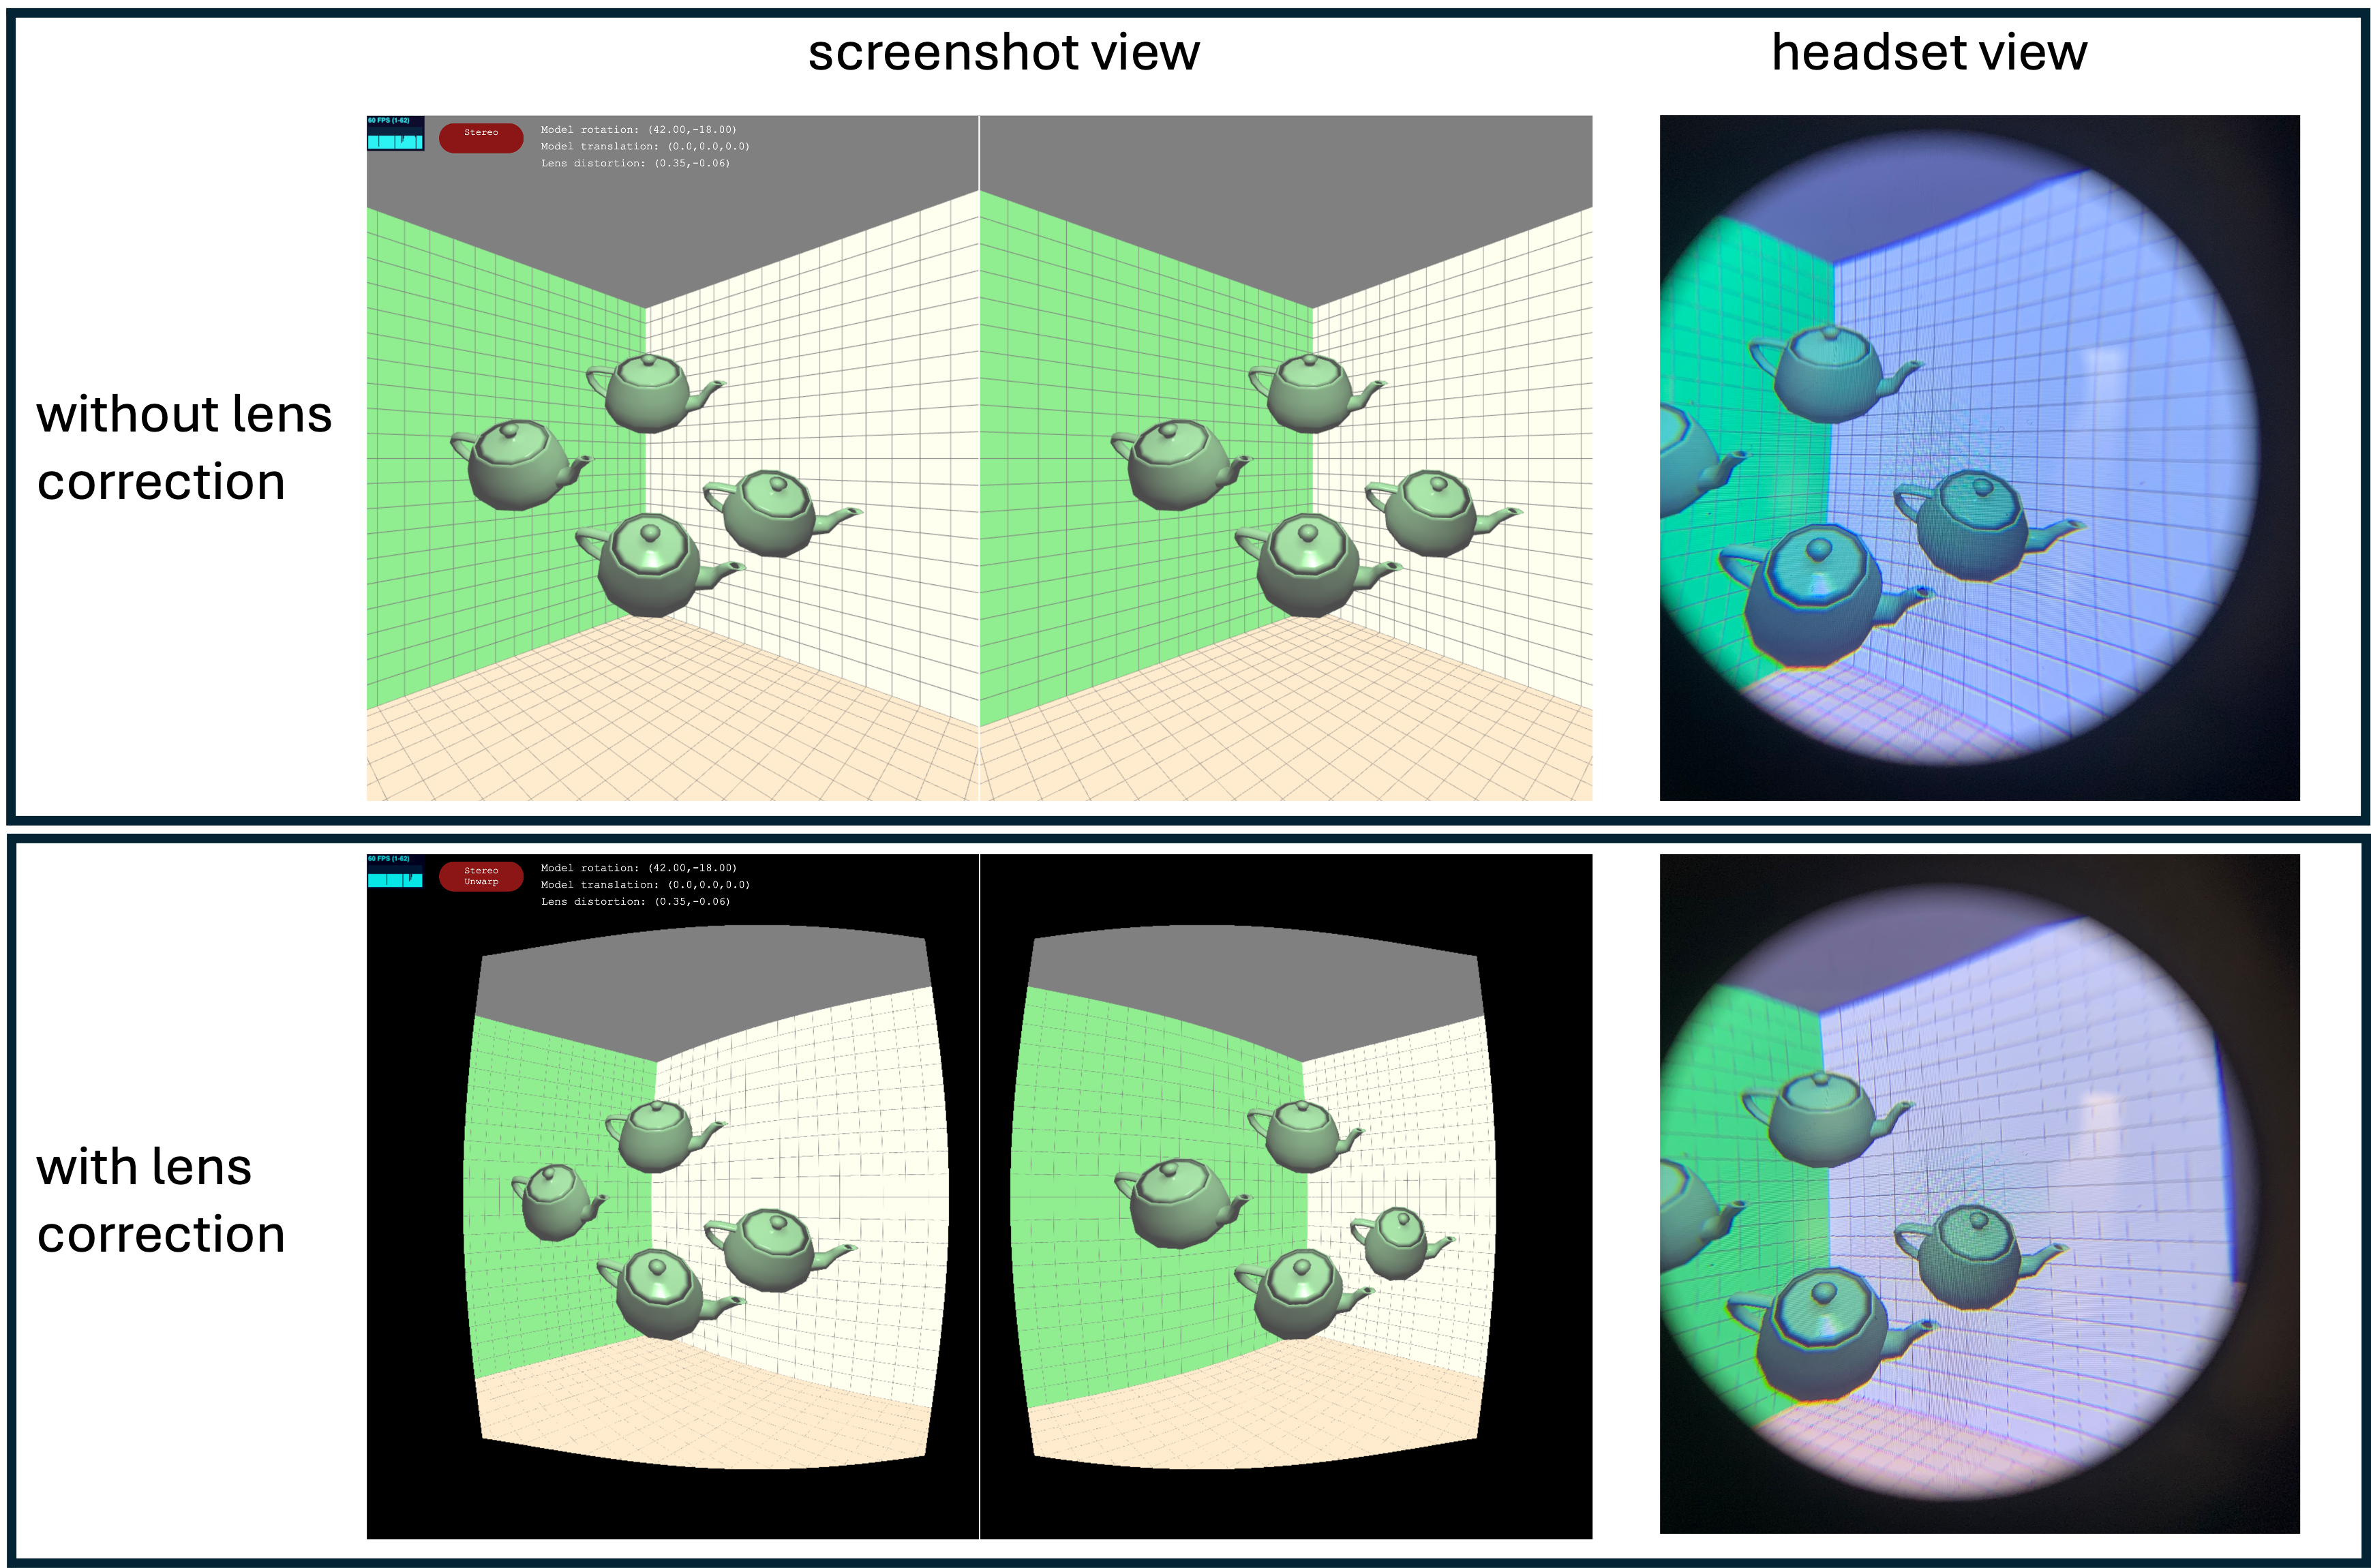
\includegraphics[width=0.8\textwidth]{lenscorrection.png}
\end{figure}


\end{document}